\documentclass[11pt,a4paper]{article}
\usepackage[utf8]{inputenc}
\usepackage{amsmath}
\usepackage{dsfont}
\usepackage{listings}
\usepackage{amsfonts}
\usepackage{amssymb}
\usepackage{tabularx}
\usepackage{enumitem}
\usepackage{algorithm}% http://ctan.org/pkg/algorithm
\usepackage[noend]{algpseudocode}% http://ctan.org/pkg/algorithmicx
\usepackage{parskip}
\usepackage{tikz}
\usepackage[margin=1in]{geometry}
\usepackage{graphicx}
\usepackage{hyperref}
\usetikzlibrary{arrows,positioning} 
\usepackage{subcaption}


\pgfarrowsdeclarecombine{ring}{ring}{}{}{o}{o}

\DeclareMathOperator{\ringarrow}{\raisebox{0.5ex}{\tikz[baseline]{\draw[ring->](0,0)--(2em,0);}}}
\DeclareUnicodeCharacter{00A0}{ }
\tikzset{
    %Define standard arrow tip
    >=stealth',
    %Define style for boxes
    observed/.style={
           circle,
           rounded corners,
           draw=black, thick,
           minimum width=2.2em,
           minimum height=2.2em,
           font=\footnotesize,
           text centered,
           },
     latent/.style={
           circle,
           rounded corners,
           draw=black, thick, dashed,
           minimum width=2.2em,
           minimum height=2.2em,
           font=\footnotesize,
           text centered,
           fill=black!10!white
           },
    target/.style={
           circle,
           rounded corners,
           draw=black, thick,
           minimum width=2.2em,
           minimum height=2.2em,
           font=\footnotesize,
           text centered,
           fill=black!20!white,
           },
    observedrect/.style={
           rectangle,
           rounded corners,
           draw=black, thick,
           minimum width=6em,
           minimum height=2em,
           font=\footnotesize,
           text centered,
           },
     targetrect/.style={
           rectangle,
           rounded corners,
           draw=black, thick,
           minimum width=6em,
           minimum height=2em,
           font=\footnotesize,
           text centered,
           fill=black!20!white,
           },
     empty/.style={
           circle,
           rounded corners,
           minimum width=.5em,
           minimum height=.5em,
           font=\footnotesize,
           text centered,
           },
    % Define arrow style
    pil/.style={
           o->,
           thick,
           shorten <=2pt,
           shorten >=2pt,},
    sh/.style={ shade, shading=axis, left color=red, right color=green,
    shading angle=45 }   
}






\newcommand{\defined}{\vcentcolon =}
\newcommand{\rdefined}{=\vcentcolon}
\newcommand{\E}[1]{\mathbb E\left[{#1}\right]}
\newcommand{\Var}{\operatorname{Var}}
\newcommand{\calF}{\mathcal F}
\newcommand{\sr}[1]{\stackrel{#1}}
\newcommand{\set}[1]{\left\{#1\right\}}
\newcommand{\ind}[1]{\mathds{1}\!\!\set{#1}}
\newcommand{\argmax}{\operatornamewithlimits{arg\,max}}
\newcommand{\argmin}{\operatornamewithlimits{arg\,min}}
\newcommand{\floor}[1]{\left \lfloor {#1} \right\rfloor}
\newcommand{\ceil}[1]{\left \lceil {#1} \right\rceil}
\newcommand{\eqn}[1]{\begin{align}#1\end{align}}
\newcommand{\eq}[1]{\begin{align*}#1\end{align*}}
\newcommand{\Ber}{\operatorname{Bernoulli}}
\newcommand{\bigo}[1]{\mathcal{O}\left( #1 \right)}
\newcommand{\bigotilde}[1]{\tilde{\mathcal{O}}\left( #1 \right)}
\newcommand{\bigtheta}[1]{\Theta\left( #1 \right)}
\newcommand{\bigthetatilde}[1]{\tilde{\Theta}\left( #1 \right)}
\newcommand{\bigomega}[1]{\Omega\left( #1 \right)}

\renewcommand{\P}[1]{\operatorname{P}\left\{#1\right\}}



\author{Finnian Lattimore}
\title{Learning how to act: making good decisions with machine learning}

\begin{document}
\def\ci{\perp\!\!\!\perp} % from Wikipedia
\newtheorem{theorem}{Theorem}[section]
\newtheorem{definition}{Definition}[section]
\maketitle

\section{Introduction}

Learning the outcome of an action is central to many real world problems. Does de-worming children in poor countries improve health and educational outcomes \cite{miguel2004,davey2015}? Would increasing the minimum wage lead to higher unemployment? Will offering this customer a discount improve my revenue? These questions are difficult as they require more than identifying a pattern in data.  There are two, very different, approaches to this problem within the machine learning community: reinforcement learning and causal inference. 

Reinforcement learning addresses the problem of learning from explicitly taking actions. There is typically some state or environment. An agent chooses an action from those available in the current state. The state then evolves stochastically as a function of the selected action and the agent receives some feedback or reward that is a function of the new state. This setting differs from the standard classification problem in that the agent must learn from feedback on the selected action, rather than being presented with the correct action for a given state. A common modelling assumption is that the state evolves only as a function of the previous state and the action chosen, and given these, is independent of the previous history of states and actions. This is known as a Markov decision process or MDP.  A particularly well studied and understood model is the singe state MDP. In this case, there are a set of actions, each associated with a fixed but unknown reward distribution and at each time step our agent selects an action and receives corresponding feedback. This is known as the multi-armed bandit problem. 

Causal inference makes use of assumptions to allow the outcome of actions to be predicted from observational data. The key to causal inference is a framework that can model how actions change the state of the world. This framework then allows us to map information collected in one setting to another. 

Both approaches can be seen as extensions to the concept of randomised controlled trials. Bandit algorithms deal with the sequential nature of the decision making process, causal inference with the problem that full randomisation is not always feasible, affordable or ethical. The similarities between the problems that these techniques have been developed to address raises the question of if there are problems best addressed by a combination of these approaches and how they can be combined. The goal of my thesis is to explore these questions. In the next sections I review the key literature in causal inference and bandits. I then present a general approach to  how causal models might be incorporated into bandit settings and conclude by demonstrating an algorithm that leverages causal assumptions to improve performance in a specific bandit setting. 

\section{Causal Inference}

\subsection{Models of causality and intervention}

Predicting the outcome of actions without explicitly taking them requires assumptions about how the actions will change the system. A very powerful and general model that underlies much of the recent work in causality is the causal bayesian network. A causal bayesian network, or directed acyclic graph (DAG), is a bayesian network in which a link $V_{i} \rightarrow V_{j}$ is defined to mean $V_{i}$ directly causes $V_{j}$. This means that if we intervene and change the value of $V_{i}$, we expect $V_{j}$ to change, but if we intervene to change $V_{j}$, $V_{i}$ will not change. More generally, if $G$ is a causal network for a distribution $P$ defined over variables $V_{1}...V_{N}$, then the distribution after an intervention where we set $X \subset V$ to $x$, denoted $do(X=x)$ is obtained by simply dropping the terms for each of the variables in $X$ from the factorization given by the network. This is referred to as the truncated product formula \cite{Pearl2000}. 

If the network contains latent (unobservable) variables we will not be able to calculate all the terms in the truncated product formula. However, it may still be possible to determine the post-interventional distribution of specific variables of interest. A general causal query $P(Y|do(X=x))$ is identifiable if it can be shown to be equivalent to an expression containing only pre-interventional quantities. This means that, asymptotically, we can obtain an unbiased estimate for the distribution after an intervention based on purely observational data. 

The do calculus is a set of three rules that allow transformations of interventional terms to non-interventional ones, given a causal graph \cite{Pearl2000}. They are derived directly from d-seperation properties of graphical models and the definition of intervention in causal DAGs. These rules are complete. A query is identifiable if and only if it can be transformed to contain only non-interventional terms via the do-calculus \cite{Shpitser2006,Huang2006}. There is an equivalent algorithm that can take any causal graph and query and determine identifiability \cite {Shpitser2008} (see \url{http://finnhacks42.github.io/causal_identify} for a javascript demonstration of this algorithm). If a query is not identifiable, it may still be possible to get bounds for causal effects, for example using instrumental variables \cite{Angrist2009} or by making additional assumptions. 

There are two other key frameworks that arise in causal inference. Counterfactuals and structural equation models.  Counterfactuals are statements about imagined or alternate realities, are prevalent in everyday language and may play a role in the development of causal reasoning in humans \cite{Weisberg2013}. Causal effects are differences in counterfactual variables; what is the difference between what would happen if we did one thing versus what would happen if we did something else \cite{Rubin1974,Rubin1978,Rosenbaum1983, Rubin2005,Rubin2008}. 

For example, if we wanted to estimate the causal effect of a medical treatment, then we might let $Y^{1}$ be a counterfactual random variable representing the (binary) potential outcome if treated. The distribution of $Y^{1}$ is the distribution we would see in the outcome $Y$ if everyone was treated. Similarly $Y^{0}$ represents the potential outcome for the placebo. The causal effect of the drug is the difference between the probability of recovery, across the population, if everyone was treated, and the probability of recovery given placebo $P(Y^{1})-P(Y^{0})$. This quantity can be estimated from observational data if we assume $X \ci Y^{0}$ and $X \ci Y^{1}$. These assumptions are referred to as ignoreability assumptions \cite{Rosenbaum1983}. They state that the treatment each person receives is independent of whether they would recover if treated and if they would recover if not treated. Graphically, this is equivalent to the assumption that there is no variable that is a parent of both the treatment $X$ and the outcome $Y$. 


Structural equation models (SEMs) describe a deterministic world, where underlying mechanisms determine the output of any process for a given input. The mechanism (but not the output) is assumed to be independent of what is fed into it. Linear structural equation models have a long history for causal estimation \cite {Wright1921,Haavelmo1943}. Mathematically, each variable is a deterministic function of its direct causes and a noise term that captures unmeasured variables. The noise terms are required to be mutually independent. If there is the possibility that an unmeasured variable influences more than one variable of interest in a study, it must be modelled explicitly as a latent (unobserved) variable. Structural equation models can be represented visually as a network. Each variable is a node and arrows are drawn from causes to their effects. If the network for a structural equation model is acyclic then it implies a recursive factorization of the joint distribution over its variables. In other words, it is a causal bayesian network. 

Remarkably for models developed relatively independently in fields with very different approaches and problems, the models we have discussed are functionally very similar. To determine if and how an interventional query can be non-parametrically identified, it is equivalent to specify assumptions graphically in terms of bayesian networks or as structural equation models or as conditional independence statements involving counterfactual variables (ignorability assumptions). 

It is possible to pose causal queries in terms of counterfactuals that are not interventional and cannot be phrased in terms of the do-notation. The scientific and philosophical validity of such counterfactual queries remains under question \cite{Dawid2000,Dawid2014}, however they are nonetheless widely posed in the form of attribution of causal effects to different pathways and mediation \cite{Pearl2014,Imai2010a,VanderWeele2011}. 

There are differences between the models we have considered when it comes to these non-interventional queries. Counterfactuals are not defined in causal bayesian networks, as they only encode information on the interventional distribution over variables.  Counterfactuals can be defined in terms of structural equation models \cite{Pearl2000} but there are subtle differences depending on the form of assumptions made. Structural equation models with independent errors allow the identification of quantities in mediation studies, which are not identifiable with the weak ignorability assumptions and cannot be tested experimentally \cite{Richardson2013}.  

In practice, differences in focus and approach across different fields eclipse the actual differences in the models. The work on causal graphical models \cite{Pearl2000,Sprites2000} focuses on non-parametric estimation in the population limit and rigorous theoretical foundations. The Neyman-Rubin framework builds on our understanding of randomized experiment and generalizes to quasi-exeperimental and observational settings, with a particular focus on non-random assignment to treatment. This research emphasises estimating average causal effects and provides practical methods for estimation, in particular, propensity scores; a method to control for multiple variables in high dimensional settings with finite data \cite{Rosenbaum1983}. In economics, inferring causal effects from non-experimental data so as to support policy decisions is central to the field. Economists are often interested in broader measures of the distribution of causal effects than the mean and make extensive use of structural equation models, generally with strong parametric assumptions \cite{Heckman2008}. In addition, the parametric structural equation models favoured in economics can be extended to analyse cyclic (otherwise referred to as non-recursive) models. 


\subsection{Discovering causal structure}

In the previous section we discussed when assumptions about the structure of the variables in a specific problem is sufficient to identify a causal effect. This approach relies on having enough prior knowledge or theory about the problem to allow you to, at least partially, specify the causal network. In this section, we consider the much harder problem of causal inference where you need to learn the network. Causal inference might seem impossible without specific assumptions about the structure of the variables involved but, amazingly, some aspects of causal structure can be determined from much more general assumptions.  

 
\subsubsection{Discovery based on conditional independence}
One general approach is to look for clues about the structure of the network in the conditional independence relations in the distribution. Assume there is some acyclic causal network $G$ that generated the distribution $P(\boldsymbol{V})$ from which our data has been sampled. Our goal is to recover the network from this data. 

Since $G$ is a bayesian network, if $Z$ d-separates $X$ and $Y$ in $G$ then $(X \ci Y|Z)$ in $P$ . However, we want to work in the other direction, from conditional independence in the distribution to the structure of the network. This requires that we assume the reverse condition: $(X \ci Y|Z)$ in $P$ must imply $Z$ d-separates $X$ and $Y$ in $G$. This assumption, commonly referred to as  \textbf{\textit{faithfulness}}, says there are no additional independence relations that are satisfied in $P$ but not in all distributions $\boldsymbol{P'}$ that are compatible with $G$. Stating that $P$ is faithful to $G$ is equivalent to $G$ is a \textbf{\textit{perfect map}} for $P$.

Faithfulness is an assumption. It does not always hold and we cannot verify it from the observational data we wish to use for causal inference. However, most distributions generated by a causal bayesian network will be faithful to that network. For faithfulness to be violated, different causal effects must exactly balance one-another out. For example, consider a simple binary variable model of chocolate consumption, income and obesity, figure \ref{fig:unfaithful}. If the coefficients in the conditional probability tables are just right then the direct effect of chocolate on obesity will exactly balance the indirect effect through income and obesity will appear independent of chocolate consumption. However, this independence is not stable. It would disappear under a small perturbation to any of the parameters.  

\begin{figure}[h]
\caption{Example of a data generated from a causal graph violating the faithfulness assumption}
\label{fig:unfaithful}
\centering
\begin{subfigure}[t]{0.99\textwidth}
\centering
\caption{True causal graph generating $P$}
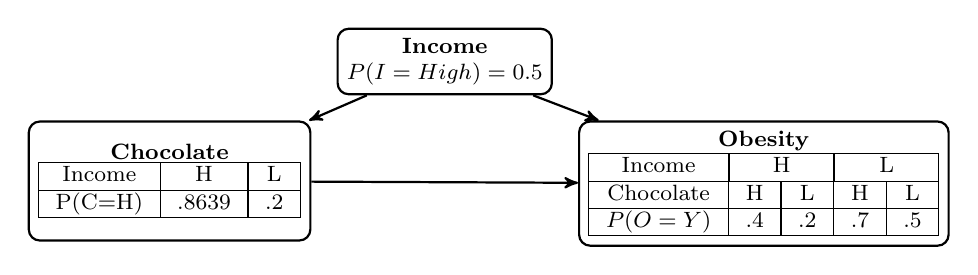
\begin{tikzpicture}[->,shorten >=0pt,shorten <=0pt,node distance=0.45cm,thick,main node/.style={observedrect}]
\node[main node, align=center,minimum height=4.3em](C){\textbf{Chocolate} \\ \begin{tabular}{| c | c | c |}
  \hline			
  Income & H & L \\
  \hline
  P(C=H) & .8639 & .2\\
  \hline
\end{tabular}};
\node[main node, above right=of C, align=center](I){\textbf{Income} \\ $P(I=High) = 0.5$};
\node[main node, below right=of I, align=center,minimum height=4.3em](O){\textbf{Obesity} \\ \begin{tabular}{| c | c | c | c | c |}
  \hline			
  Income & \multicolumn{2}{| c |}{H} & \multicolumn{2}{| c |}{L} \\
  \hline
  Chocolate & H & L & H & L \\
  \hline
  $P(O=Y)$ & .4 & .2 & .7 & .5 \\
  \hline
\end{tabular}};
\path[]
	(I) edge (C) edge (O)
	(C) edge (O);
\end{tikzpicture}
\vspace{1em}
\end{subfigure}

\begin{subfigure}[b]{0.99\textwidth}
\centering
\caption{Perfect map for $P, \;(C \ci O)$}
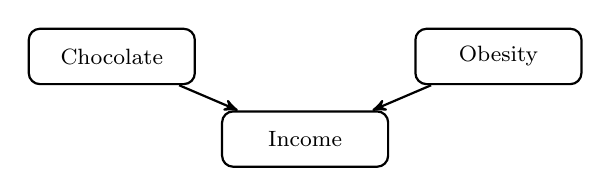
\begin{tikzpicture}[->,shorten >=0pt,shorten <=0pt,node distance=0.45cm,  thick,main node/.style={observedrect}, shaded/.style={latent}]
\node[main node](C){Chocolate};
\node[main node, below right=of C](I){Income};
\node[main node, above right=of I](O){Obesity};
\path[]
	(C) edge (I)
	(O) edge (I);
\end{tikzpicture}
\end{subfigure}
\end{figure}

Given the faithfulness assumption, our causal discovery problem reduces to finding the set of bayesian networks that have exactly the dependency structure as we observe in $P$. A wide range of algorithms have been developed based on this key observation, see table \ref{table:discovery_algorithms}. Constraint based methods such as the PC algorithm \cite{Sprites2000}, FCI algorithm \cite{Sprites2000} and RFCI algorithm \cite{Colombo2012}, perform sequential conditional independence tests and eliminate inconsistent graphs. Search and score based methods, such as GES \cite{Chickering2002}, search over the space of graphs and score them according to how well they fit the independences given a complexity penalising prior. Constraint based methods are faster, particularly for sparse graphs, but can lack robustness as errors in early conditional independence tests can propagate. Search and score based methods are more robust for small samples sizes but difficult to scale to larger graphs. This has led to the development of hybrid approaches, such as the MMHC algorithm \cite{Tsamardinos2006}. A key component of causal discovery is the ability to do high dimensional non-parametric conditional independence tests. Developments in kernalized conditional independence tests,\cite{Gretton2008,Zhang2012} have made this possible.


\begin{table}[h]
\centering
\caption{A comparison of key causal discovery algorithms}
\label{table:discovery_algorithms}
\renewcommand{\arraystretch}{1.5}
\begin{tabular}{| c | c | p{4cm} | c | c |}
\hline
  \textbf {Alg.} &\textbf{ Method }& \textbf{Scales (num.vars) }& $\sim $ \textbf {Vars} & \textbf {Latent }  \\
  \hline
  PC & Constraint based & Worst case exponential, polynomial for sparse graphs & 5000 & No  \\ 
  \hline
  FCI & Constraint based & Worst case exponential, polynomial variant FCI+ for sparse graphs & 30 & Yes\\
  \hline
  RFCI & Constraint based & ? & 500 & Yes  \\
  \hline
  GES & Search \& Score  & Worst case exponential & 50 & No  \\
  \hline
  MMHC & Hybrid & ? & 5000 & No  \\
 \hline
\end{tabular}
\end{table}

 

If the end goal of causal discovery is to estimate causal effects, then it may not be necessary to learn the entire graph, only the subset of the graph surrounding target variables of interest. Such local causal discovery techniques can be scaled to problems with many more variables \cite{Aliferis2002}. Once a set of causal graphs has been identified, causal effects of interest can be bounded by combining the results for the all the networks. This procedure is the IDA algorithm \cite{Maathuis2009} and has been found to outperform standard regularization techniques at finding causal effects in a high-dimensional yeast gene expression data set \cite{Maathuis2010}. An implementation is available in the R package pcalg \cite{Kalisch2012}

\subsubsection{Discovery with functional models}
All of the algorithms we have considered so far return a Markov equivalence class. They cannot distinguish between two models that result in the same set of conditional independence relations. Consider the very simple case where we have only two variables and the only possible causal structures are $X \rightarrow Y$ or $Y \rightarrow X$. These models have the same dependency structure but in one case $P(Y|do(X)) = P(Y|X)$ and in the other $P(Y|do(X)) = P(Y)$. No algorithm relying purely on conditional independence relations can separate these two cases.

One solution is to utilize structural equation models to specify additional assumptions. For example, if we assume that noise is additive, such that $X \rightarrow Y \implies Y = f(X)+\epsilon$, then this will only be invertible such that $X = g(Y) + \epsilon'$ for specific pairs of functions $f$ and noise distributions $\epsilon$. Thus in general we will be able to identify the causal direction \cite{Hoyer2009}. This can be extended to post-non-linear additive noise, $Y = h(f(X)+ \epsilon)$, \cite{Zhang2008a}. These techniques can also be applied over more than two variables \cite{Peters2014}.

A more general approach is to leverage the assumption that the functions are independent of inputs \cite{Janzing2012a}. This leads to the idea that $P(X)$ and $P(Y|X)$ are independent if $X \rightarrow Y$ but not if $Y \rightarrow X$. \cite{Janzing2012} propose testing for this by applying both semi-supervised and standard techniques to estimate $P(Y|X)$. Semi-supervised methods, which utilize additional points from $P(X)$ to learn $P(Y|X)$ should only be able to outperform standard methods if $Y \rightarrow X$. 

Finally, rather than explicitly developing an algorithm based on a specific asymmetry between cause and effect, \cite{LopezPaz2014} propose learning what causality looks like from data. They take as input a dataset where each row of data is itself a dataset in which either $X \rightarrow Y$ or $Y \rightarrow X$ and a corresponding label. Estimates of the distributions $P(X)$, $P(Y)$ and $P(X,Y)$ for each row are then mapped to features in some kernel space via mean kernel embeddings and finally a standard classification algorithm can be trained to learn the labels. New datasets, where the direction of causality is unknown, are then simply mapped to the kernel space and the causal direction is classified according to the trained classifier. In practice, the classifier is trained mostly on simulated data as it is difficult to find a sufficient set of causal problems with only two variables, where the direction of causality is known. 

\section{Multi-armed Bandits}

In its classic formulation \cite{Robbins1952} the (stochastic) K-armed bandit describes a sequential decision making problem, with $K$ possible actions or arms. Each arm $i$ is associated with a fixed but unknown reward distribution $\nu_i$ \footnote{In order to obtain regret bounds, some assumptions are required on the distributions $\nu_i$. It sufficient to assume they are sub-gaussian}.  For each timestep $t$ upto a horizon $T$ the learner selects an action $I_t \in \set{1...K}$ and receives a reward, $g_{I_t,t}$, sampled i.i.d from $\nu_i$. The goal of the learner is to maximize the total reward they receive. This problem introduces the fundamental exploration-exploitation trade-off. The learner must balance playing arms that have yielded good results previously with exploring arms about which they are uncertain. 

The performance of bandit algorithms is generally described by the (pseudo) regret, $R(T)$. This is the difference between the expected reward obtained by the algorithm and the expected reward of selecting the best action in every timestep. 

\eqn {
R(T) = max_{\set{i=1...K}} \E{\sum_{t=1}^T g_{i,t}} - \E{\sum_{t=1}^T g_{I_t,t}}
}

If we let $\mu_i = \E{\nu_i}$ denote the expected reward for each arm $i$ and $\mu^* = max_{\set{i=1...K}}(\mu_i)$ denote the reward for the best arm:

\eqn {
R(T) = T\mu^* - \sum_{t=1}^T E[\mu_{I_t}] 
} 

An algorithm is learning if it obtains regret that is sublinear in $T$. The lower bound on the worst case regret for any algorithm (stochastic or adversarial) for the K-armed bandit problem is  $\bigomega{\sqrt{TK}}$ \cite{Auer1995}.

A key algorithm for stochastic bandits, with tractable analysis and strong performance guarantees, is the UCB algorithm \cite{Auer2002}. They key to this algorithm is that it keeps track of an upper confidence bound (hence UCB) on the expected reward for each arm and selects the arm with the highest one. This balances exploration and exploitation as an arm with a high upper confidence bound must have either a high expected reward or large uncertainty on the expected reward. Assume for notational simplicity that $\mu_1 > \mu_2 > ... > \mu_K$, such that $\mu^* = \mu_1$, and let $\Delta_i = \mu_i - \mu^*$ be the sub-optimality for each arm. The (problem dependent) regret for UCB is bounded by: 

\eqn {
R^{ucb}(T) \in \bigo{\sum_{i=2}^K \frac{1}{\Delta_i}\log(T)}
}

This bound blows up as differences $\Delta_i \rightarrow 0$, however the regret itself does not - since although we may not be able to distinguish arms with very small $\Delta_i$ from the optimal arm, we also do not lose much by selecting them. In the worst case, $R^{ucb}(T) = \bigo{\sqrt{TK\log(T)}}$ \cite{Bubeck2012}. Subtle modifications to the UCB algorithm can eliminate the logarithmic term in this worst case regret bound. This yields $R^{ucb}(T) = \bigo{\sqrt{TK}}$ and closes the gap with the worst case lower bound \cite{Audibert2009,Lattimore2015}, whilst retaining a good problem dependent bound of the form achieved by UCB \cite{Lattimore2015}.

Adversarial bandits are an alternate, widely studied, setting that relaxes the assumption that rewards are generated stochastically. Instead, simultaneously with the learner selecting an action $I_t$, a potentially malicious adversary selects the reward vector $\boldsymbol{g}_t$. As in the stochastic setting, the learner then receives reward $g_{I_t,t}$. The seminal algorithm for adversarial bandits is Exp-3, which, like UCB, obtains regret $\bigo{\sqrt{TK\log(T)}}$ regret \cite{Auer1995}. Optimal algorithms, with $R(T) = \bigo{\sqrt{TK}}$, have also been demonstrated for the adversarial setting \cite{Audibert2009}.

Another problem that has attracted a lot of recent attention \cite{Bubeck2009,Audibert2010,Gabillon2012,Karnin2013} within the multi-armed bandit framework is \textit{pure exploration} or \textit{best arm identification}. In this setting, the horizon $T$ represents a fixed budget for exploration after which the algorithm outputs a single best arm $i$. The performance of the algorithm is measured by the simple regret; the expected difference between the mean reward of the (truly) optimal arm and the mean reward of the arm selected by the algorithm, $R_s(T) = \mu^* - \E{\mu_i}$ . This problem arises naturally in applications where there is a testing or evaluation phase, during which regret is not incurred, followed by a commercialization or exploitation phase. For example, many strategies might be assessed via simulation prior to one being selected and deployed. The simple regret for a K-armed bandit is lower bounded by $\bigo{\sqrt{K/T}}$ \cite{Bubeck2009}.


The classic multi-armed bandit is a powerful tool for sequential decision making. However, the regret grows linearly with the number of (sub-optimal) actions and many real world problems have large or even infinite action spaces. This has led to the development of a wide range of models that assume some structure across the reward distributions for different arms, for example generalized linear bandits \cite{filippi2010parametric}, dependent bandits \cite{Pandey2007}, X-armed bandits \cite{Bubeck2010} and gaussian process bandits \cite{srinivas2009gaussian}, or that consider more complex feedback, for example the recent work on graph feedback \cite{Mannor2011,Lelarge2012,Alon2013,Buccapatnam2014,Kocak2014,Alon2015} and partial monitoring \cite{Piccolboni2001,Bartok2014}. 

\section{Unifying the frameworks}

A natural way to connect the causal framework with the bandit setting is to model the problem as a causal directed acyclic graph. Each possible assignment of variables to values is an action (bandit arm). See figure \ref{fig:unify_frameworks} for a simple example. The reward could be a general function of the action selected and the final state of the graph. However for simplicity, we will consider the reward to be the value of a single specified node minus the cost of the selected action. The number of actions or arms grows exponentially with the number of variables in the graph, making it important to use algorithms that take account of the graph structure to reduce the search space. 

Modelling a problem as a causal graph only makes sense when rewards are generated stochastically - since causal graphs fundamentally model probability distributions over variables. Thus the connection is to stochastic bandit problems (although adversarial bandits algorithms may be applied to stochastic problems). 


\begin{figure}[h]
\caption{A simple causal graphical model and corresponding complete action space. A and B represent binary variables that can be intervened on and Y represents the reward.}
\label{fig:unify_frameworks}
\centering
\begin{subfigure}[c]{0.3\textwidth}
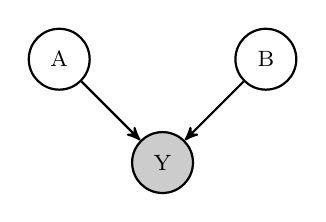
\begin{tikzpicture}[->,shorten >=0pt,shorten <=0pt,node distance=3em,thick,main node/.style={observed}, tg/.style={target}]
\node[main node](1){A};
\node[tg, below right=of 1](2){Y};
\node[main node, above right=of 2](3){B};
\path[]
	(1) edge (2)
	(3) edge (2);
\end{tikzpicture}
\end{subfigure}
\begin{subfigure}[t]{0.4\textwidth}
Actions = \begin{tabular}{|c|}
	\hline
  do(A=0,B=0) \\
  do(A=0,B=1) \\
  do(A=1,B=0) \\
  do(A=1,B=1) \\
  \hline
  do(A=0) \\
  do(A=1) \\
  do(B=0) \\
  do(B=1) \\
  do() \\
  \hline
\end{tabular}
\end{subfigure}
\end{figure}



If we begin by considering the case where the causal graph is known, problems then take on characteristics of different bandit settings depending on the assumptions we make about what subset of actions can be taken, what variables are observable and whether they are observed before or after an action is selected. 

If feedback is received only on the reward node then the do-calculus can be applied to eliminate some actions immediately, before any experiments are performed and then a standard bandit algorithm can be run on the remaining actions. See figure \ref{fig:cholesterol_graph} as an example. 

\begin{figure}[h]
\caption{Example causal graph (based on \cite{Koller2009}) where the outcome of interest (reward) is cholesterol level . The do-calculus can be applied to eliminate some actions immediately without the need to do any experiments. For example, no actions involving 'Test Result' need to be considered and interventions on 'Diet' do not need to be considered in conjunction with any other variables.}
\label{fig:cholesterol_graph}
\centering
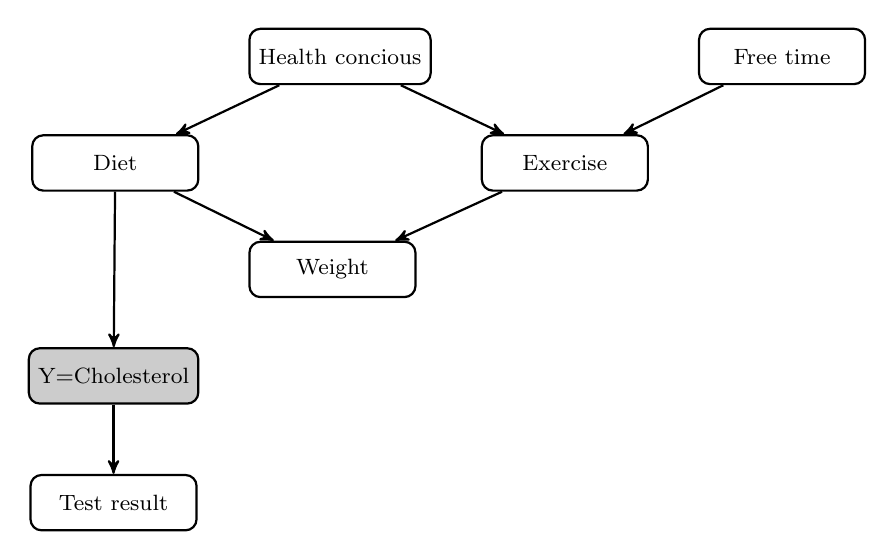
\begin{tikzpicture}[->,shorten >=0pt,shorten <=0pt,node distance=2.5em,thick,node/.style={observedrect},tg/.style={targetrect}]
\node[node](1){Health concious};
\node[node, below left=of 1](2){Diet};
\node[node, below right=of 1](3){Exercise};
\node[node, below right=of 2](4){Weight};
\node[tg,below left=of 4](5){Y=Cholesterol};
\node[node, below =of 5](6){Test result};
\node[node, above right=of 3](7){Free time};
\path[]
	(1) edge (2) edge (3)
	(2) edge (4) edge (5)
	(3) edge (4)
	(5) edge (6)
	(7) edge (3);
\end{tikzpicture}
\end{figure}

If we receive feedback on additional nodes, the problem can be more interesting. In addition to being able to eliminate some actions prior to sampling any data as in the previous case, taking one action may give us some information on actions that were not selected. Consider again the model in figure \ref{fig:unify_frameworks}. The causal structure implies: 

\eqn {
P(Y|do(A = 0)) &= P(Y|do(),A = 0) \\
&= P(Y|do(B=0),A=0)P(B=0)+P(Y|do(B=1),A=0)P(B=1) 
}

Thus we gain information about the reward for the action $do(A=0)$ from selecting the action $do()$ or $do(B = b)$ and then observing $A = 0$.  

We only get this form of side information for actions that don't specify the value of every variable, ie those in the bottom half of the table in figure \ref{fig:unify_frameworks}. Since the reward distribution for actions that set a subset of the variables is the result of marginalizing out other variables, they can only be optimal if they have lower cost. So if the cost of all actions is constant (no matter how many variables must be set), then the problem has the same characteristics as if only the reward node were observable.

If the information on the value of additional nodes is available prior to selecting an action the problem resembles a contextual bandit. For example if we observe $A = 0$ then, in deciding between the actions $do(B=0)$ and $do(B=1)$, we would want information on $P(Y|A=0,B=0)$ and $P(Y|A=0,B=1)$.  Note, side information can still arise if we learn the value of some variables prior to selecting an action and some afterwards. 


\subsection{Incorporating side information induced by casual graph}

As a first step towards more general problems, we develop and evaluate a bandit algorithm that incorporates the side information induced by a specific causal graph. 

Assume we have a known causal model with binary variables $\boldsymbol{X} = \{X_{1}..X_{N}\}$ that independently cause a target variable of interest $Y$, figure \ref{fig:causalStructure}. This is an expansion of the model shown in figure \ref{fig:unify_frameworks}. We can run sequential experiments on the system, where at each timestep $t$ we can either do nothing, $do()$, or select a single variable, $X_i$, on which to intervene, $do(X_{t,i} = J_t)$, and subsequently observe the complete result, $(\boldsymbol{X}_{t},Y_{t})$. 

As an example, consider a farmer wishing to optimize the yield of her crop. She can invest in a green house to control temperature, a watering system to control soil moisture, fertilizers to set soil nutrients, etc. We assume only a single intervention is feasible due to cost and that each of these variables are independent of one-another (this may not always be the case - temperature could be related to rainfall for example). After having selected which variable to control, she plants her crops and observes the values of the remaining input variables and the yield. This repeats across many growing seasons, and the goal is to maximize the total cumulative yield.

\begin{figure}[h]
\centering
\caption{Assumed Causal Structure}
\label{fig:causalStructure}
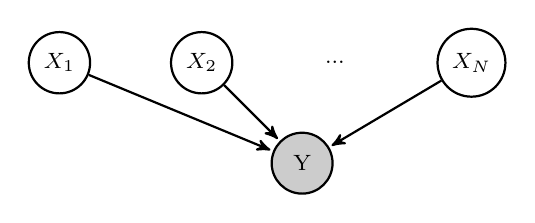
\begin{tikzpicture}[->,>=stealth',shorten >=1pt,auto,node distance=1cm,
  thick,main node/.style={observed}, hidden/.style={empty},tg/.style={target}]

 %nodes
\node[main node](1){$X_{1}$};
\node[main node, right=of 1](2){$X_{2}$};
\node[hidden, right=of 2](3){$...$};
\node[main node, right=of 3](4){$X_{N}$};
\node[tg, below right=of 2](5){Y};
 \path[every node/.style={font=\sffamily\small}]
    (1) edge (5)
    	(2) edge (5)
    (4) edge (5);
	
\end{tikzpicture}
\end{figure}


Let $\boldsymbol{q} \in [0,1]^N$ be a fixed vector where $q_i = P(X_i = 1)$. In each time-step $t$ upto a known horizon $T$:
 
\begin{enumerate}
\item The learner chooses an $I_t \in \set{0,\ldots, N}$ and $J_t \in \set{0,1}$, where $I_t = 0$ represents $do()$.

\item Variables not set by the learner take their values probabilistically according to $\boldsymbol{q}$ 
\eq{
X_{t,i} = \begin{cases}
\sim \Ber(q_i) &\text{if } i \neq I_t \\
J_t & \text{otherwise}\,.
\end{cases}
}
\item The learner observes $(\boldsymbol{X}_{t},Y_{t})$ and receives reward $Y_t \sim \Ber(r(\boldsymbol{X}_{t}))$ where $r:\set{0,1}^N \to [0,1]$ is unknown and arbitrary. 
\end{enumerate}

The problem could be treated as a standard bandit problem with $K = 2N + 1$ arms, 

\eq {
\{do(), do(X_1=0), do(X_1 = 1)\;\; ... \;\;do(X_N = 1)\}
}

yielding a regret $\bigo{\sqrt{TN}}$. However, this doesn't leverage the side information induced by the causal structure: 

\eqn {
\label{eq:observe}
P(Y_t|do(X_{i,t} = j)) &= P(Y_t|do(),X_{i,t} = j) \\
\label{eq:estimation_transfer}
&= P(Y_t|do(X_{l,t}=0),X_{i,t}=j)(1-q_l)+P(Y_t|do(X_{l,t}=1),X_{i,t}=j)q_l 
}

The hardness of this problem depends strongly on the vector $\boldsymbol{q}$. This is intuitive from a consideration of the extreme cases. If $\boldsymbol{q} = \boldsymbol{0}$ (or $\boldsymbol{1}$), then half of the actions we wish to explore will only occur if we explicitly select them. For these actions we get no side information by playing other actions. So at best we could expect a factor of two improvement over simply running a standard bandit algorithm. If $\boldsymbol{q} = \boldsymbol{\frac{1}{2}}$, the observe action, $do()$, effectively becomes a revealing action and we would anticipate obtaining a regret with minimal dependence on the number of variables $N$. 

We consider a simple explore-exploit based algorithm, that will explore for $h$ timesteps, sampling actions in a way that depends on $\boldsymbol{q}$. We then select the arm with the highest expected reward for the remaining $T-h$ time steps. During the exploration phase, we will balance purely observing, $I_t = 0$, which takes advantage of equation \ref{eq:observe} to reveal the reward for frequently occurring arms, with explicit sampling of infrequently occurring arms. 

Without loss of generality, we can assume $q_i \in [0,\frac{1}{2}]$ and $q_1 \leq q_2 ... \leq q_N$. Let:

\eqn {
m \in [2,N] = \set{m:q_m > \frac{1}{m}}
}

$m$ is a measure of the number of infrequently occurring arms. If the problem is completely balanced $q_1...q_N = \frac{1}{2}$ then $m = 2$. If the problem is completely unbalanced, $q_1...q_N = 0$ then $m=N$.  Let $q_{ij} = \P{X_i = j}$ and $\mu_{ij} = P(Y|do(X_i = j))$.


Suppose we select $I_t = 0$ for the first $h/2$ timesteps. This is at worst half the optimal. We use these observations to estimate the rewards for all the frequently occurring arms, $\set{do(X_i = 0) \; \forall i}$, and $\set{X_i = 1:i \geq m}$ 

\eqn {
\hat{\mu}_{ij} = \frac{\sum_{t=1}^{h/2}\ind{Y_t=1,X_{t,i}=j}}{\frac{h}{2}q_{ij}}
}

We then explicitly play each of the $m$ infrequently occurring arms $\frac{h}{2m}$ times and estimate their rewards as:

\eqn {
\hat{\mu}_{ij} = \frac{2m}{h}\sum_{t = 1}^{h/2m}\ind{Y_t = 1|X_i=j}
}

We then simply play the arm with the highest estimated reward for the remaining $T-h$ timesteps. We can show that we can select an $h$ (based on $T$, $N$ and $m$) that leads to worst case regret $R_T = \bigotilde{T^{2/3}m^{1/3}}$. This result can still be obtained in the case where $\boldsymbol{q}$ is unknown and must be learned during the exploration time. Comparing this to the standard bandit regret, $R_T = \bigo{\sqrt{TK}}$, we expect the causal algorithm to do better if $m < \frac{K^{3/2}}{\sqrt{T}}$. We can also show that the simple regret $R_s \in \bigotilde{\sqrt{m/T}}$. If $m << K$, this represents a significant improvement over standard bandit setting. \footnote{ $\bigotilde{.}$ and $\bigthetatilde{.}$ suppress polylogarithmic factors}


In this algorithm, we have only used the side information provided by the $do()$ action about other actions. Since the $do()$ action fully reveals the value of alternate actions we could have incorporated this information via the graph feedback model \cite{Mannor2011}, where at each timestep the feedback graph $G_t$ is selected stochastically, dependent on $\boldsymbol{q}$, and revealed after an action has been chosen. The feedback graph is distinct from the causal graph. A link $A \rightarrow B$ in $G_t$ indicates that selecting the action $A$ reveals the reward for action $B$. For this specific problem, $G_t$ will always be a star graph with the action $do()$ connected to half the remaining actions. The Exp3-IX algorithm \cite{Kocak2014} was developed for the adversarial version of this problem and has regret $\bigo{\sqrt{\bar{\alpha}T}}$, where $\bar{\alpha}$ is the average independence number of $G_t$. In our case $\bar{\alpha} = \frac{N}{2}$ so we again obtain the regret of the standard bandit algorithm. The issue here is that a malicious adversary can select the same graph each time, such that the rewards for half the arms are never revealed by the informative action. This is equivalent to a, nominally, stochastic selection of feedback graph where $\boldsymbol{q} = \boldsymbol{0}$

\cite{Lelarge2012} consider a stochastic version of the graph feedback problem, but with a fixed graph available to the algorithm before it must select an action. In addition, their algorithm is not optimal for all graph structures and fails, in particular, to provide improvements for star like graphs as in our case. \cite{Buccapatnam2014} improve the dependence of the algorithm on the graph structure but still assume the graph is fixed and available to the algorithm before the action is selected. 

More generally, assuming causal structure creates more complex types of side information, such as that shown in equation \ref{eq:estimation_transfer}. In this case, selecting one action does not fully reveal an alternate action but provides some information towards an estimate. The quality of the estimate notably depends not only on the number of times that action was selected. For example, to get a good estimate for $X_1 = 1$ by intervening on $X_2$ requires us to sample both $X_2=0$ and $X_2=1$, in proportions dependent on $q_2$. This more complex side information does not fit within the graph feedback framework.

Partial monitoring is a very general framework for for decoupling the feedback from the action and reward. It can be used to classify problems into one of four categories, trivial with no regret, easy with $R_T = \bigthetatilde{\sqrt{T}}$ , hard with $R_T = \bigtheta{T^{2/3}}$ and hopeless with $R_T = \bigomega{T}$ \cite{Bartok2014}. Partial monitoring algorithms yield results that are optimal with respect the the horizon $T$ but not other parameters, such as $K$, which is the key focus of incorporating causal structure. 



\subsection{Open questions}

There are many open questions still to be addressed. For the specific setting described above I need to derive lower bounds for the worst case regret so as to determine how close the current approach is to optimal. 

It is clearly desirable to obtain an algorithm that could be generalized to an arbitrary causal graph. This will likely require the development of a bandit algorithm that can leverage more complex forms of side information like that in equation \ref{eq:estimation_transfer}, in addition to an efficient algorithm for eliminating actions that need not be considered at all.

Another open class of problem to consider are cases where the causal structure is not (fully) known and also needs to be learnt within the online setting. 

\section{Paid work statement}
I am not currently undertaking or planning to undertake any paid work.


\bibliographystyle{unsrt}% Select the citation style e.g. ieeetr
\bibliography{../library}% write the directory to the .bib file
\end{document}




